\section{4 cycles}

The 5-types
\begin{enumerate}
  \renewcommand*{\labelenumi}{(\alph{enumi})}%
  \renewcommand*{\theenumi}{(\alph{enumi})}%

  \item $1$ edge on the cycle/fence
  \label{t:1}
  \item 2 consecutive edges on the cycle/fence
  \label{t:2cons}
  \item 2 non-consecutive edges on the cycle fence
  \label{t:2alt}
  \item 3 edges on the cycle/fence
  \label{t:3}
  \item Just a vertex on the cycle/fence
  \label{t:0}
\end{enumerate}

Note that type \ref{t:2alt} and \ref{t:3} can't occur on the cycle since the give a chord.

\subsection{On the cycle}

\paragraph{Type \ref{t:1}}
This is a \emph{short chord}


\paragraph{Type \ref{t:2cons}}

\paragraph{Type \ref{t:2alt}}

\paragraph{Type \ref{t:3}}

\paragraph{Type \ref{t:0}}




\subsection{On the fnce}


\paragraph{Type \ref{t:1}}
This is a \emph{short chord}


\paragraph{Type \ref{t:2cons}}

\paragraph{Type \ref{t:2alt}}

\begin{figure}[h]
  \centering
  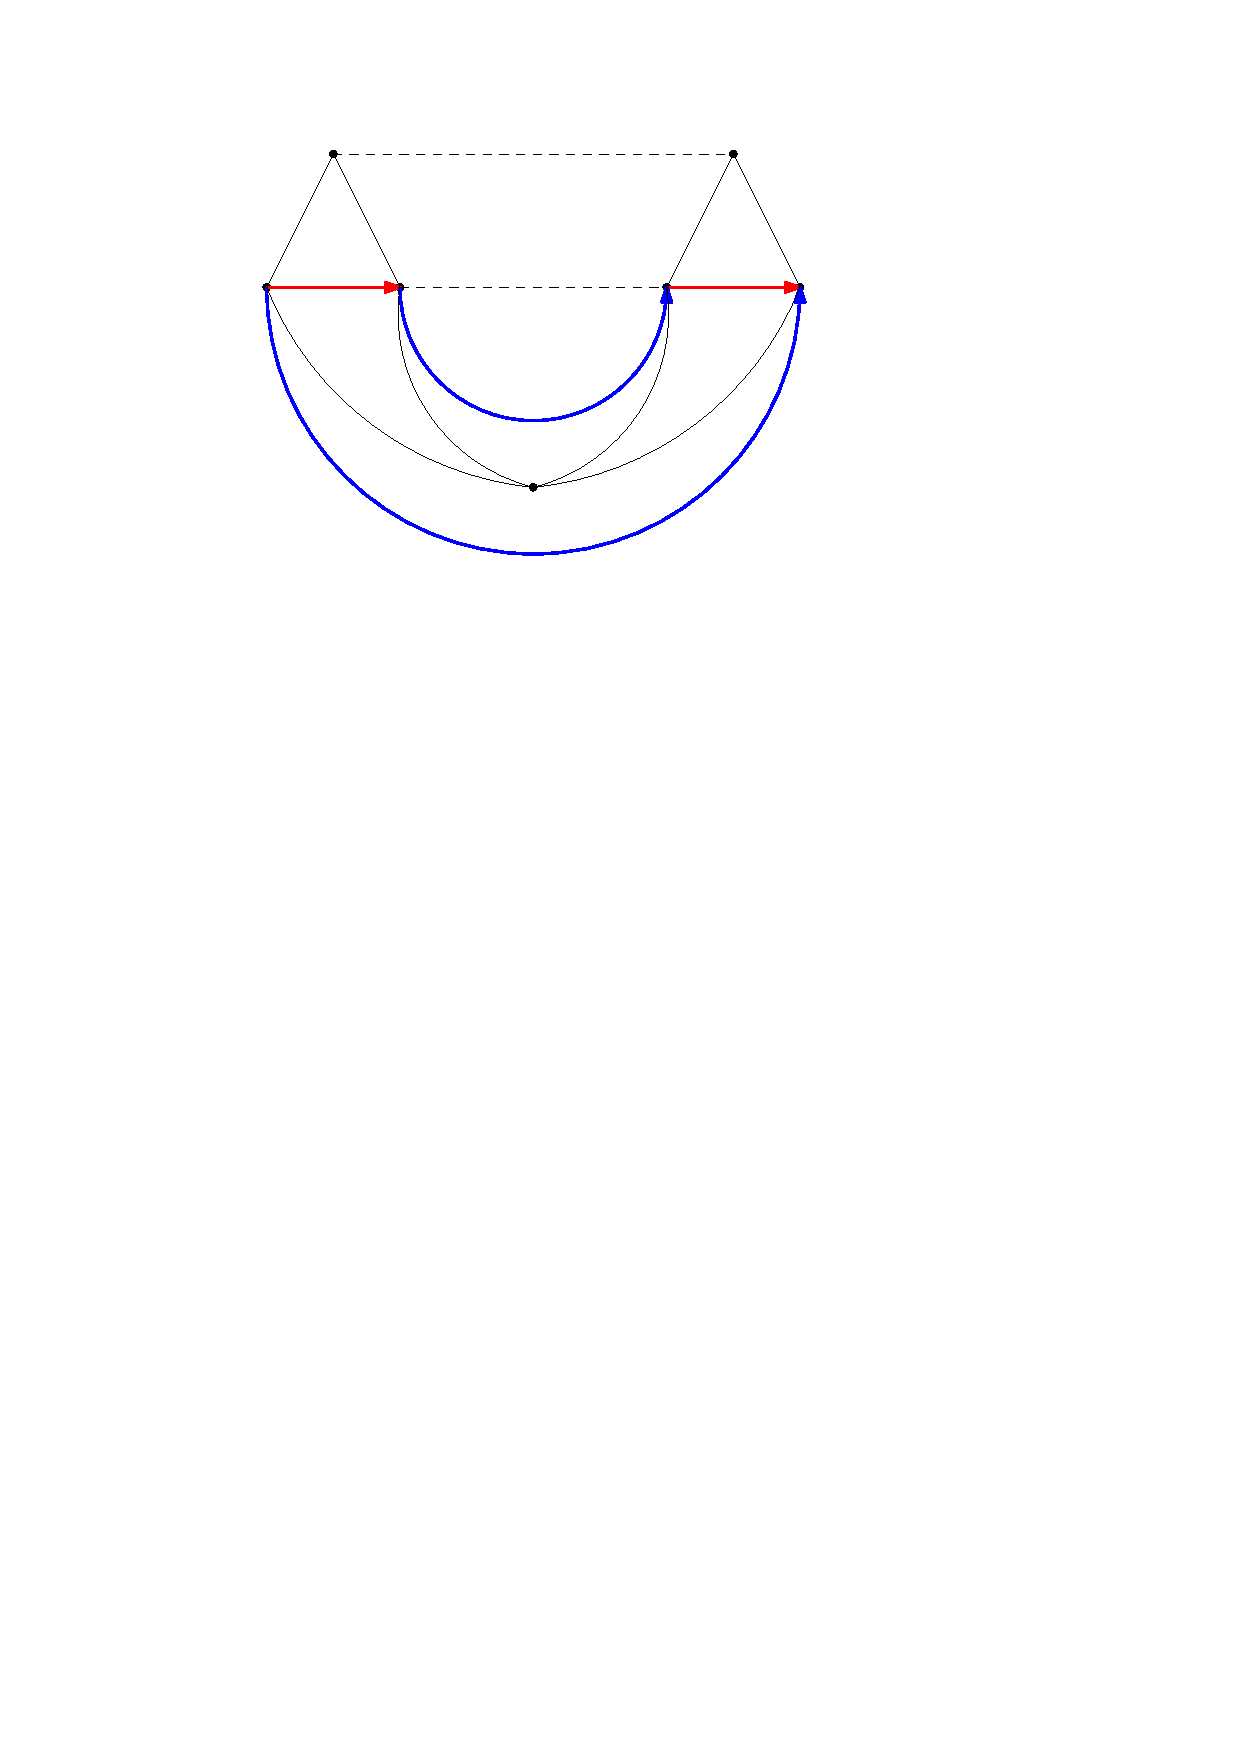
\includegraphics[scale=1]{4cycles/img/fence_c}
  \caption{}
  \label{fig:}
\end{figure}

\paragraph{Type \ref{t:3}}

\subsubsection{Type \ref{t:3}}

\begin{figure}[h]
  \centering
  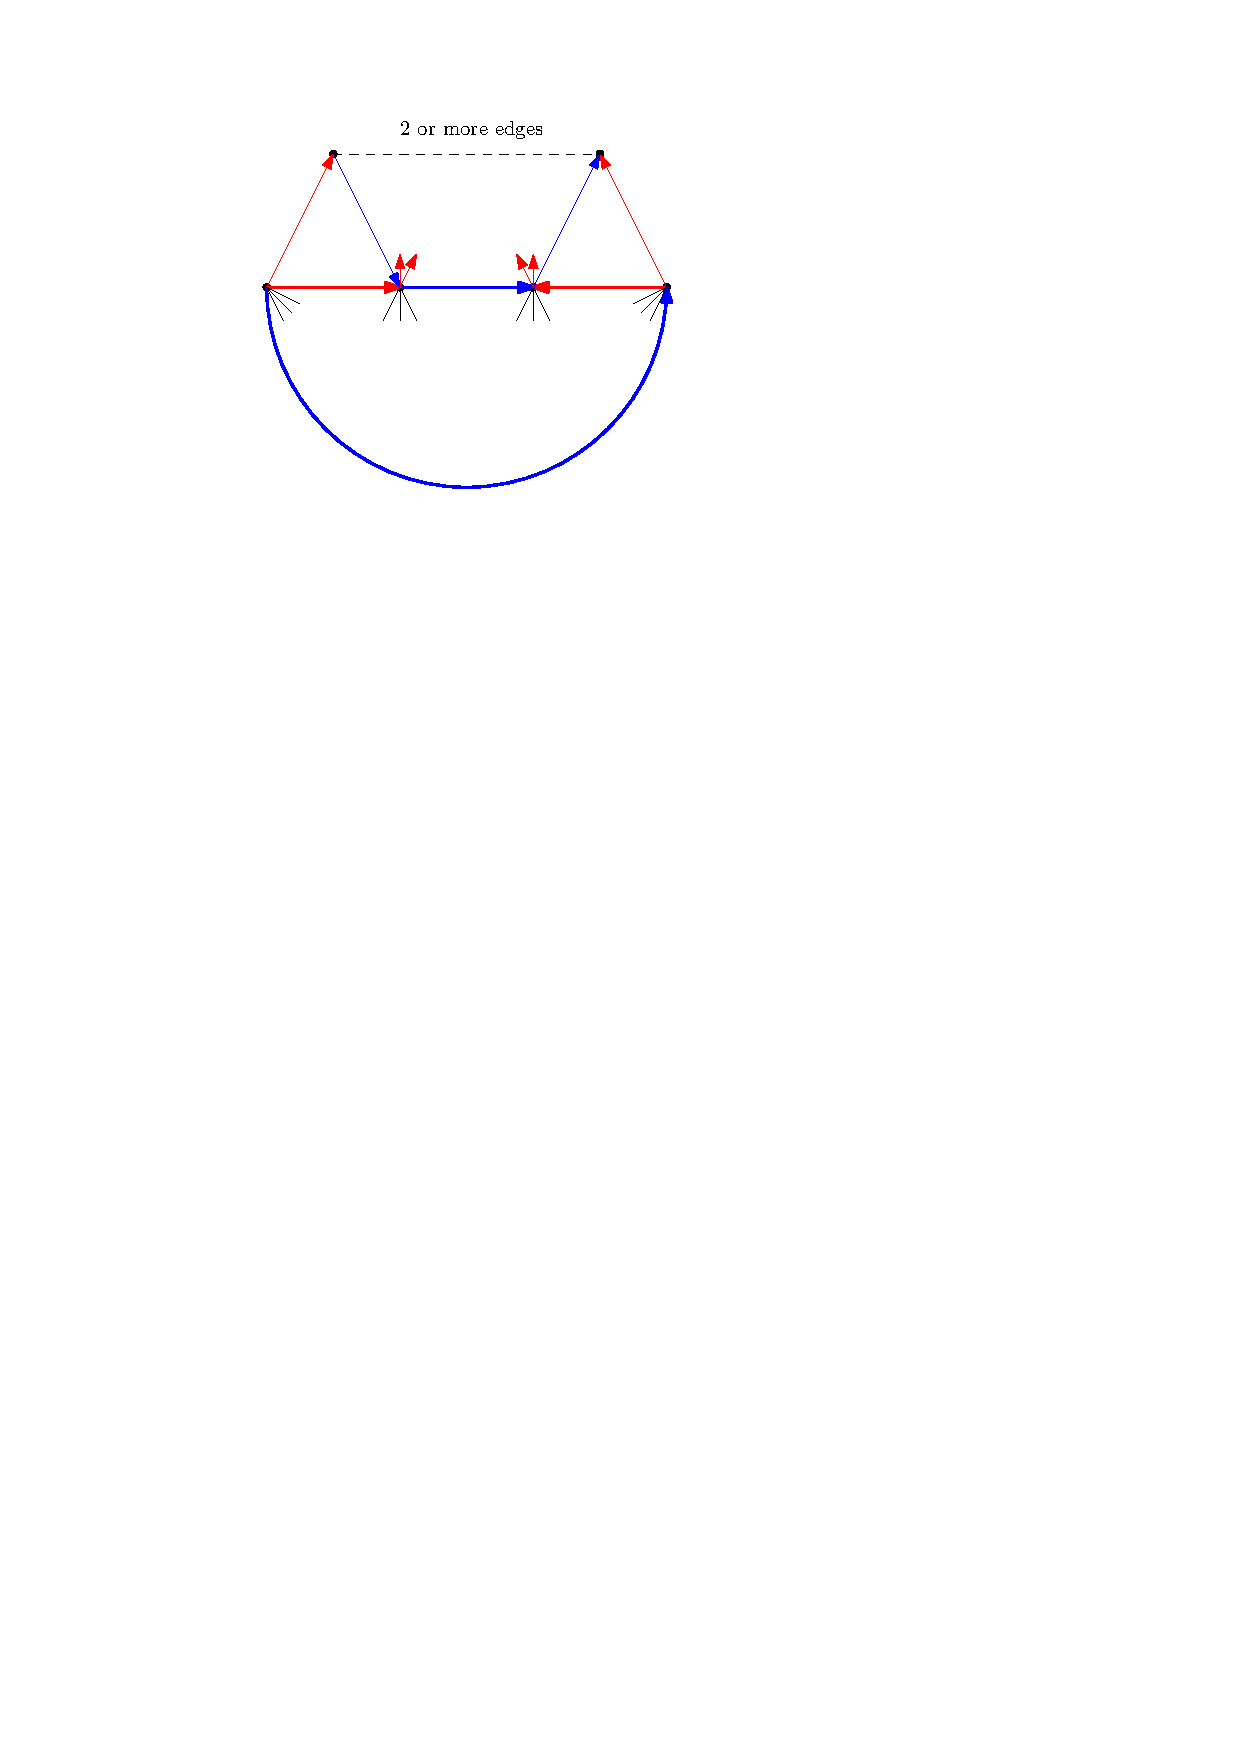
\includegraphics[scale=1]{4cycles/img/fence_d}
  \caption{}
  \label{fig:}
\end{figure}

\paragraph{Type \ref{t:0}}


\subsection{On the inside of a chord}
seems to go okay

\subsection{Adjecent 4-cycles}
